\chapter{Implementation}

\begin{minipage}{12cm}

\dirtree{%
	.1 /.
	.1 bin\DTcomment{binaries}.
	.1 data\DTcomment{filebased MDPs}.
	.1 examples\DTcomment{example applications}.
	.1 src.
	.2 mdpsolve\DTcomment{library code}.
	.3 Evaluations\DTcomment{policy evaluation modules}.
	.3 Parser\DTcomment{mdp parsing modules}.
	.3 Policies\DTcomment{policy improvement modules}.
	.3 Solvers\DTcomment{solving algorithms modules}.
	.1 tests\DTcomment{test environment}.
}
\end{minipage}
\section{Interface}

Considering the requirements from \autoref{goals} the header \emph{interface.hpp} shall be provided to the application:

\begin{lstlisting}
struct Params{
	std::string mdp_filepath_;
	std::string module_parser_;
	std::string module_eval_;
	std::string module_policy_;
	std::string module_solver_;
	std::size_t solver_iteration_cnt_;
};
/*
Solve mdp that is defined in a file on the filesystem
*/
std::unique_ptr<Policy> solve_filebased_mdp(const Params& params);
/*
Solve mdp that has been defined by the application
*/
std::unique_ptr<Policy> solve_external_mdp(Model& model,const Params& params);

\end{lstlisting}

The functionality provided in the interface is implemented in \emph{solve.cpp}. 

\section{Model}

The model class is the core element of library because it holds information about the MDP to be solved. It is initialized using the default constructor and a Parser-Module (\autoref{chaptermodule}) is parsing the MDP definition from the input file to the model class. Since memory for the model class members has to be allocated dynamically, the parsing model class object offers a public method to allocate the required memory for the object. Once the Parser-Module has determined the size of the state and action space, \emph{setArrays()} can be called to initialize the array data structures of the state transition matrix and the reward matrix. A method to validate the model data is offered by the model class and is called by the Parser-Module to abort parsing if an inconsistency has been detected. 

The state transition matrix and reward matrix are represented using the \emph{Array3d template class} (\autoref{array}).
Both matrices are used to look up transition probabilities and rewards.

\begin{equation}
P_a(s,s') = state\_transition\_matrix[a,s,s']
\end{equation}

\begin{equation}
R_a(s,s') = reward\_matrix[a,s,s']
\end{equation}



\section{Modules}
\label{chaptermodule}

In order to achieve a high level of extensibility this base class acts a blue print for classes to read or write the model. Using this common interface enables easy integration which is described in detail in \autoref{integration}. The module class consists of a protected constructor to set its most important member: a reference to the model. This class is totally independent from the new C++20 feature which is also called Modules. 

Four interfaces inherit from the module class and describe different types of modules:

\begin{itemize}
	\item Parser (parser.hpp)
	\item Policy (policy.hpp)
	\item Evaluation (evaluation.hpp)
	\item Solver (solver.hpp)
\end{itemize}

\begin{figure}[ht]
	\centering
	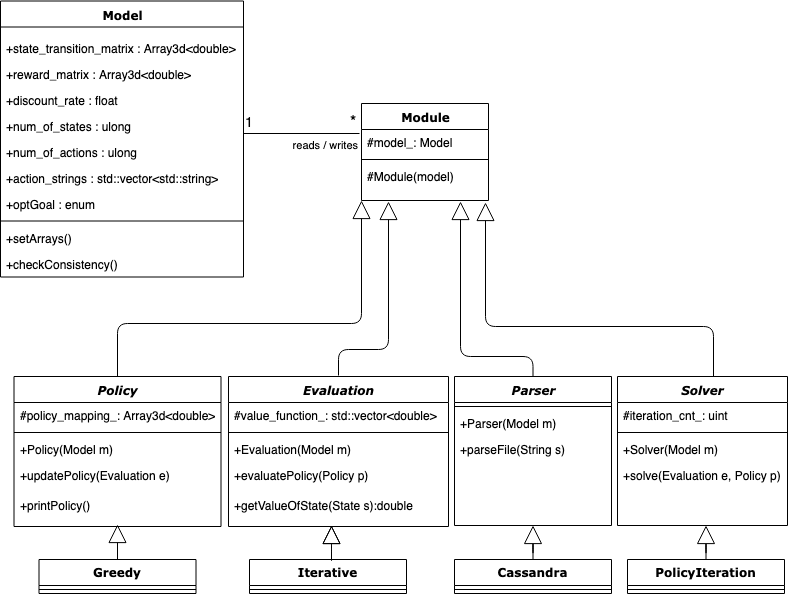
\includegraphics[width=.9\textwidth]{images/Modules.png}
	\caption{\label{fig:bild2}Model and Modules}
	\label{Modules}
\end{figure}

The abstract \emph{Parser} class acts as an interface for concrete Parser implementations. There exist several file formats to describe MDPs. For the sake of a running example, a rudimentary implementation to parse \emph{POMDP} file format \autocite{Cassandra} is provided. This format is referred to in the code by the name of the author: \emph{Cassandra}. This class only parses a minimal subset of the POMDP grammar and lacks validation. 

The abstract \emph{Policy} class as a interface for different variations of \emph{policy improvement}. The \emph{policy mapping} member is a multdimensional matrix represented as an \emph{Array3d Object} (\autoref{array}) in order to both support deterministic policies and stochastic policies. A method is provided to select an action given a certain state. This is needed by Evaluation-implementations. The policy class is also used as a return type for the external interface of the library. This way an external application can use the reference to directly integrate the optimal strategy for the environment. 

The abstract \emph{Evaluation} class is an interface for different implementatons of policy evaluation. A simple form of policy evaluation is provided in the library: \emph{iterative policy evaluation}. This method applies \autoref{valuefunction} to update the value of each state. 

The \emph{Solver} interface and base class provides a general solve method. Solving algorithms combine policy evaluation and policy improvement in different ways to find the optimal policy. \emph{Policy iteration} is implemented as an example.

Classes implementing the required interface of these interfaces are located in the according subdirectories. 

\section{Module factory}
\label{integration}

In order to minimize the amount of effort to integrate and instantiate additional functionality, a factory (\emph{factory.hpp}) is implemented. The implementation for the factory and constructor is based on the lecture material \autocite{lectureFactory}. A factory pattern combined with self registering types enables integration of new functionality without adding any references in existing code. To ensure scalability it has been decided to use a template class as a factory and instantiate a factory for each module category (Parser, Policy, Evaluation, Solver). Based on the factory template, customized factories can be implemented if needed. The factory template class is designed as a singleton and follows the \emph{construct on first use idiom}. A given name defined in the constructor of a new module is used as an identifer within the factory to decide which object to create. Using multiple factories reduces the risk of name conflicts between modules.  Alternatively a global factory could have been used with the category name encorporated in the given name. A global factory would have offered lower flexibility and was disregarded. 

The constructor (\emph{constructor.hpp})is a template class and used as a type in the factory as well as a base class for concrete constructors. The concrete constructor class has to override the virtual create(..) method and register to its factory.
In order to minimize necessary code changes when including a new type, it has been decided to implement self registering types by instantiating a static constructor object. This has drawbacks when it comes to building since the static objects and new functionality remains unreferenced and dropping it has to be avoided as described in \autoref{build}. 
It has been decided that the advantage of not having to touch any existing code overweighs. 

\autoref{SolverFactory} depicts a factory of type Solver and a new Solver implementation ("NewSolver"). 

\begin{figure}[ht]
	\centering
	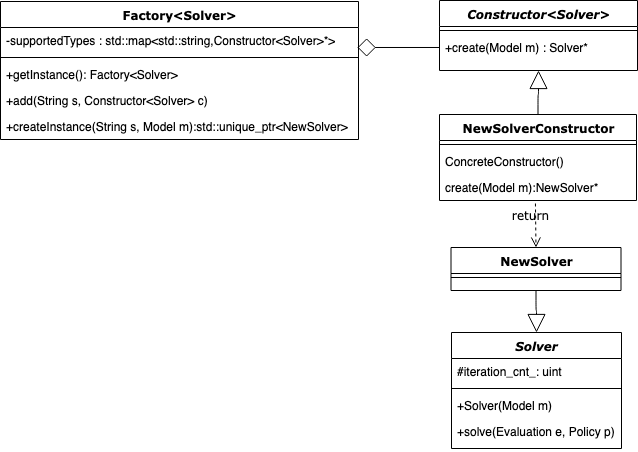
\includegraphics[width=.8\textwidth]{images/SolverFactory.png}
	\caption{\label{fig:bild2}Solver factory}
	\label{SolverFactory}
\end{figure}

For each new module two classes have to be added:

\begin{itemize}
	\item Class with new functionality, inheriting from module class or a module category
	\item Constructor class, inheriting from Constructor template class
\end{itemize}

After the constructor is succesfully registered, the factory can call its create(..) method which returns a pointer to the new object. In order to avoid memory leaks, the factory creates a std::unique\_ptr object for the returned pointer. The factory then returns this std::unique\_ptr to the caller which will also transfer exclusive ownership. By using a unique\_ptr the caller does not have to handle deletion of the created object. The drawback of this solution is that if the caller happens to need a std::shared\_ptr for distribution the construction of it comes at the cost of a dynamic memory allocation. 
Since the unique\_ptr is more lightweight and no use case for a shared\_ptr could be identified, it has been favored. 

Both constructor and factory enforce that new classes inherit from the module class when using the module factory. This is achieved with a new C++20 feature named \emph{concepts}. Concepts ease the implementation of compile-time validation of template arguments and provide meaningful compile errors to the user. 
Following concept enforces the template argument to inherit from the module class:

\begin{lstlisting}
template <typename T>
concept ModularType  = std::is_base_of<Module,T>::value;
\end{lstlisting}

The concept of a \emph{ModularType} is used for the factory and constructor template classes. 

\section{Array3d}
\label{array}
To process the state transition matrix and reward structure of a MDP, a multidimensional array implementation is needed. One option is to use \emph{std::vector} holding another std::vector for the two-dimensional case. The std::vector class manages its own resources following RAII (Resource Acquisition Is Initialization)making this a simple and robust solution but performance-wise there is a drawback. The memory for this nested structure will be fragmented which will slow down access. 
In order to make use of std::vector without causing fragmented memory the \emph{Array3d} template class (\emph{array3d.hpp}) acts as a wrapper to a one-dimensional std::vector. The () operator accepts three indices and maps those to the 1d std:.vector member. The wrapper performs a boundary check on the 3d indices. If successful, the access to the 1d vector can be performed without the need for a boundary check. This enhances the performance.  

The Array3d template class does not constrain the template argument in any way. Since internally a std::vector object with the same type has to be instantiated, the restrictions that the vector class provides are sufficient. 





\section{Example}

A sample mdp is provided in the \emph{data} directory: "4x3.95.POMDP" \autocite{Cassandra}. The mdp describes a 4x3 gridworld (\autoref{maze}) with a blocked cell (\#), a cell with high positive reward(+1) and a cell with high negative reward(-1). The cell field is not in the state space and the states of the cells with high rewards cause the transition to a random state (restarting). The action space consists of four move actions: north(N), south(S), east(E), west(W). Moving into the wall or into the blocked cell will return the same state. With a probability of 20\% an move into a direction which is perpendicular to the intended direction is happening. The mdp is used with full observability. 

The example application (directory: \emph{examples}) performs 20 steps of policy iteration on the defined mdp and then prints the expected optimal policy (\autoref{mazesolution}).

\begin{table}[]
	\centering
	\begin{tabular}{|c|c|c|c|}
		\hline
		-0.04 & -0.04                      & -0.04 & \cellcolor[HTML]{9AFF99}+1 \\ \hline
		-0.04 & \cellcolor[HTML]{C0C0C0}\# & -0.04 & \cellcolor[HTML]{FFCCC9}-1 \\ \hline
		-0.04 & -0.04                      & -0.04 & -0.04                      \\ \hline
	\end{tabular}
	\caption{4x3.95.POMDP by Stuart Russel}
	\label{maze}
\end{table}

\begin{table}[]
	\centering
	\begin{tabular}{|c|c|c|c|}
		\hline
		E & E                          & E & \cellcolor[HTML]{9AFF99}N \\ \hline
		N & \cellcolor[HTML]{C0C0C0}\# & N & \cellcolor[HTML]{FFCCC9}N \\ \hline
		N & E                          & N & W                         \\ \hline
	\end{tabular}
	\caption{Solution of the example mdp}
	\label{mazesolution}
\end{table}
